% Created 2022-02-28 Mon 16:10
% Intended LaTeX compiler: pdflatex
\documentclass[presentation,aspectratio=169]{beamer}
\usepackage[utf8]{inputenc}
\usepackage[T1]{fontenc}
\usepackage{graphicx}
\usepackage{grffile}
\usepackage{longtable}
\usepackage{wrapfig}
\usepackage{rotating}
\usepackage[normalem]{ulem}
\usepackage{amsmath}
\usepackage{textcomp}
\usepackage{amssymb}
\usepackage{capt-of}
\usepackage{hyperref}
\usepackage{khpreamble}
\usepackage{amssymb}
\usepgfplotslibrary{groupplots}
\newcommand*{\shift}{\operatorname{q}}
\DeclareMathSymbol{\Omega}{\mathalpha}{letters}{"0A}% italics
\DeclareMathSymbol{\varOmega}{\mathalpha}{operators}{"0A}% upright
\providecommand*{\upOmega}{\varOmega}% for siunitx
\usepackage[binary-units=true]{siunitx}
\usepackage{circuitikz}
\usetheme{default}
\author{Kjartan Halvorsen}
\date{\today}
\title{Actuators}
\hypersetup{
 pdfauthor={Kjartan Halvorsen},
 pdftitle={Actuators},
 pdfkeywords={},
 pdfsubject={},
 pdfcreator={Emacs 26.3 (Org mode 9.4.6)}, 
 pdflang={English}}
\begin{document}

\maketitle

\section{Mechanical requirements}
\label{sec:orgaf21477}

\begin{frame}[label={sec:org30366de}]{Mechanical requirements}
\end{frame}
\begin{frame}[label={sec:orgc9667c5}]{Mechanical energy}
From Encyclopaedia Britannica
\begin{quote}
\alert{Mechanical energy} The sum of kinetic energy (the energy in movement) and the potential energy (energy stored in a system due to the position of its parts).
\end{quote}

\[ E_M = \underbrace{K}_{\text{Kinetic energy}} + \underbrace{U}_{\text{Potential energy}}\]

\pause
A point mass \(m\) with velocity \(v\) at a height \(h\) above the reference level, has mechanical energy \(E_M = \frac{1}{2}mv^2 + mgh\).

\begin{center}
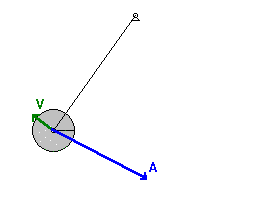
\includegraphics[height=0.3\textheight]{../../figures/pendulum.png}
{\footnotesize Source: Hubert Christiaen, wikipedia}
\end{center}
\end{frame}


\begin{frame}[label={sec:org2fde100}]{Work}
From Encyclopaedia Britannica
\begin{quote}
\alert{Work} In physics, the measure of \alert{transfer of energy} when an object is diplaced \alert{a certain distance} by an \alert{external force} which has a component in the direction of the displacement..
\end{quote}
\end{frame}

\begin{frame}[label={sec:orgcf01b17}]{Work}
\begin{center}
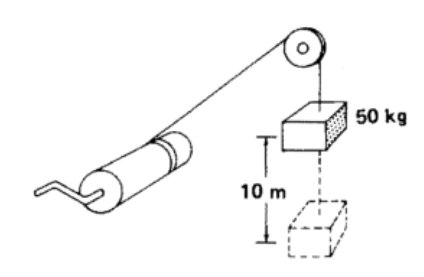
\includegraphics[height=0.6\textheight]{../../figures/pulley-block-50kg.png}
\end{center}

\alert{Activity} A mass of \unit{50}{\kilogram} is lifted a distance of \unit{10}{\meter}. What is the work done?
\end{frame}



\begin{frame}[label={sec:org4e6340d}]{Power}
\alert{Definition} The time-derivative of work.
\end{frame}

\begin{frame}[label={sec:orgb29c678}]{Power}
\begin{center}
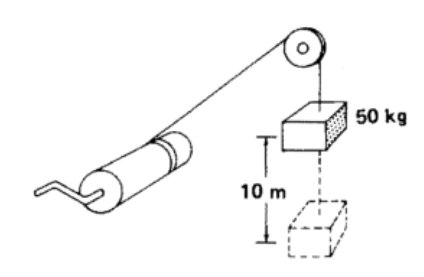
\includegraphics[height=0.6\textheight]{../../figures/pulley-block-50kg.png}
\end{center}

\alert{Activity} A mass of \unit{50}{\kilogram} is lifted a distance of \unit{10}{\meter} in 5 seocnds. What is the average power required?
\end{frame}

\begin{frame}[label={sec:org85fe442}]{Power and acceleration}
   \begin{center}
\begin{tikzpicture}

  \begin{scope}[scale=0.3, xshift=4cm]
  \node[anchor=south,] {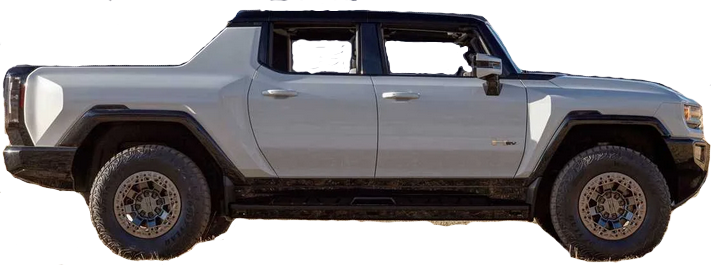
\includegraphics[width=3cm]{../../figures/hummer-ev.png}};
    \draw[thin, ] (-8,2) -- (-6,2);
    \draw[thin, ] (-9,3) -- (-6.5,3);
  \end{scope}

  \draw[->,semithick] (-.5,0.16) -- (8,0.16);
\end{tikzpicture}
\end{center}


\alert{Activity} The new Hummer EV has a mass of \(m=\unit{5000}{\kilogram}\), and can accelerate from \unit{0 - 100}{\kilo\meter\per\hour} in three seconds. What is the average power required to achieve this (ignoring wind- and rolling resistance)?
\end{frame}

\begin{frame}[label={sec:orgaa9bffa}]{Power in rotating systems}
\alert{Torque} multiplied with \alert{angular velocity}

\[ P = T\omega\]
\end{frame}

\begin{frame}[label={sec:org3ef0d64}]{Moment of inertia}
\begin{columns}
\begin{column}{0.38\columnwidth}
\begin{center}
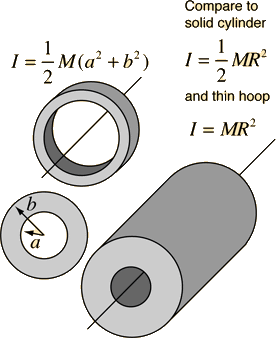
\includegraphics[height=0.6\textheight]{../../figures/moment-of-inertia-cylinder.png}
{\footnotesize Source: Georgia State University}
\end{center}
\end{column}

\begin{column}{0.72\columnwidth}
Moment of inertia is a parameter in Newton's law that determines

\begin{itemize}
\item the tendency of a body to resist angular acceleration:
\[ \textcolor{red!80!black}{J} \dot{\omega} = \sum T_i \]
\item the kinetic energy of a body rotating at a certain angular velocity:
\[ K = \frac{1}{2}\textcolor{red!80!black}{J}\omega^2.\]
\end{itemize}
\end{column}
\end{columns}
\end{frame}



\begin{frame}[label={sec:org07221cf}]{Power and torque requirements for an elevator}
\begin{columns}
\begin{column}{0.38\columnwidth}
\begin{center}
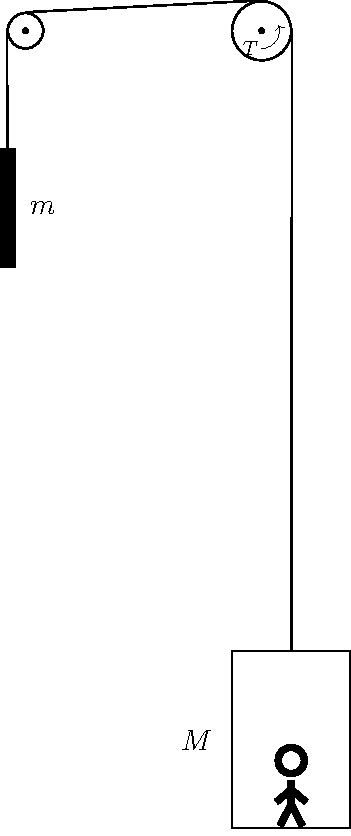
\includegraphics[height=0.8\textheight]{../../figures/mech-elevator}
\end{center}
\end{column}

\begin{column}{0.72\columnwidth}
An elevator with mass \(M=\unit{1000}{\kilogram}\), and a counterweight with mass \(m=\unit{800}{\kilogram}\) are connected by a wire which runs over a pulley with radius of \(r=\unit{0.4}{\meter}\). An electric  motor is connected to the pulley via a transmission with gear ratio of 12:1 (12 revolutions of the motor for each revolution of the pulley). The motor has a moment of inertia of \(J_m = \unit{0.3}{\kilogram\meter\squared}\). The inertia of the pulley can be ignored.

 \alert{Activity} 
\alert{(a)} At what angular velocity is the motor rotating when the elevator is ascending at \unit{4}{\meter\per\second}? \alert{(b)} Determine the power and the motor torque necessary to lift the elevator at \unit{4}{\meter\per\second} (assuming no friction). \alert{(c)} The elevator takes two seconds to reach the velocity \unit{4}{\meter\per\second} from zero. During this time, the elevator has moved up \unit{4}{\meter}. Determine the average power and torque during the start.
\end{column}
\end{columns}
\end{frame}

\section{The DC motor}
\label{sec:org10af172}
\begin{frame}[label={sec:org9cc0a64}]{The DC motor}
\begin{center}
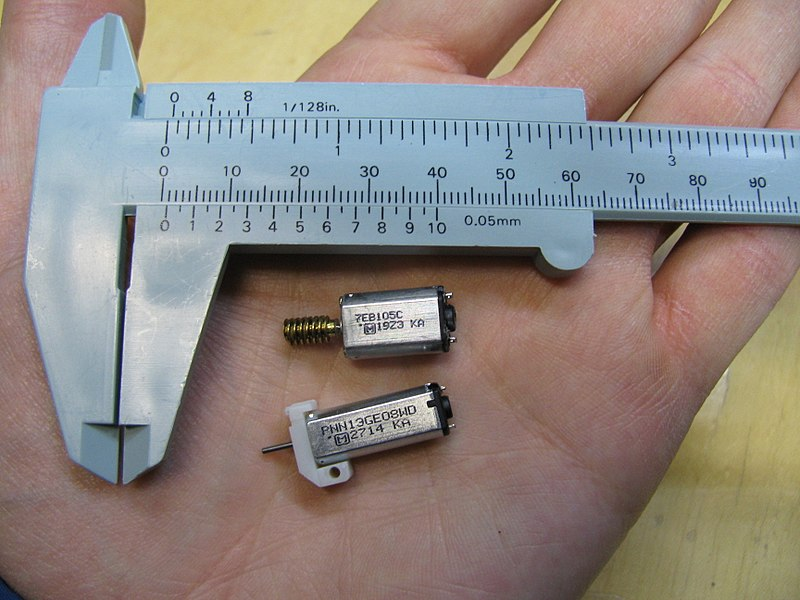
\includegraphics[height=0.6\textheight]{../../figures/wiki-small-dc-motor.jpg}
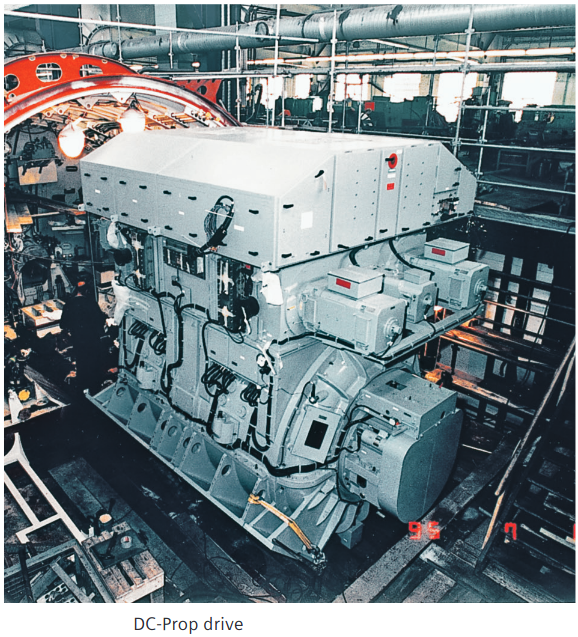
\includegraphics[width=0.6\textheight]{../../figures/Siemens-DC-prop.png}\\
{\footnotesize Source: Wikipedia \hspace*{3cm} Source: Siemens AG}
\end{center}
\end{frame}


\begin{frame}[label={sec:org75da967}]{Force on an electrical conductor in a magnetic field}
\begin{center}
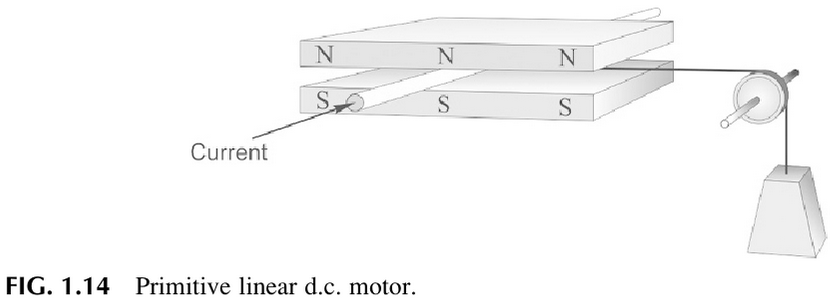
\includegraphics[width=0.4\linewidth]{../../figures/HD-fig1_14.png}
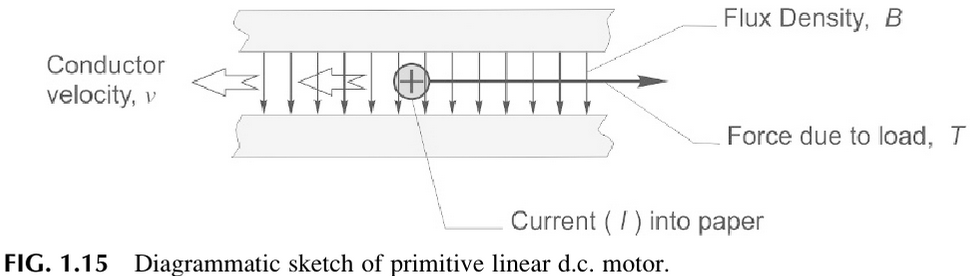
\includegraphics[width=0.53\linewidth]{../../figures/HD-fig1_15.png}
\end{center}


\begin{block}{Source}
\begin{center}
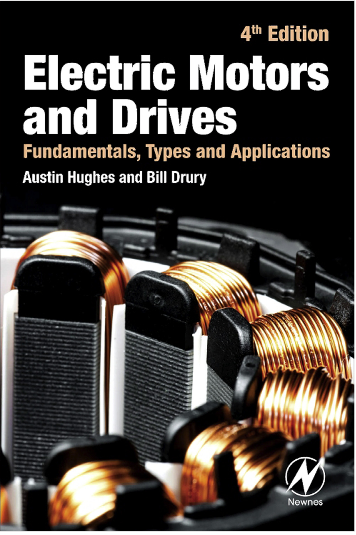
\includegraphics[width=0.2\linewidth]{../../figures/textbook.png}
\end{center}
\end{block}
\end{frame}


\begin{frame}[label={sec:org9e38f71}]{Force on an electrical conductor in a magnetic field}
\begin{center}
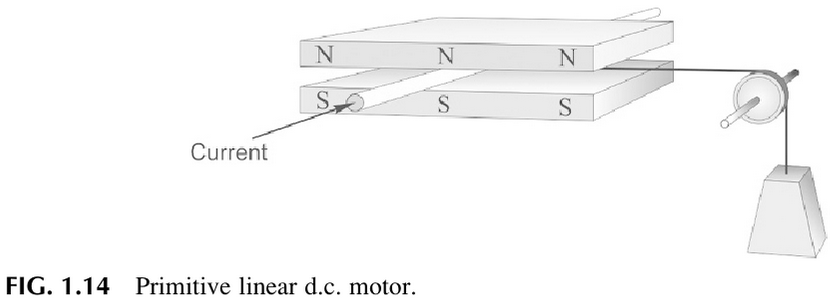
\includegraphics[width=0.4\linewidth]{../../figures/HD-fig1_14.png}
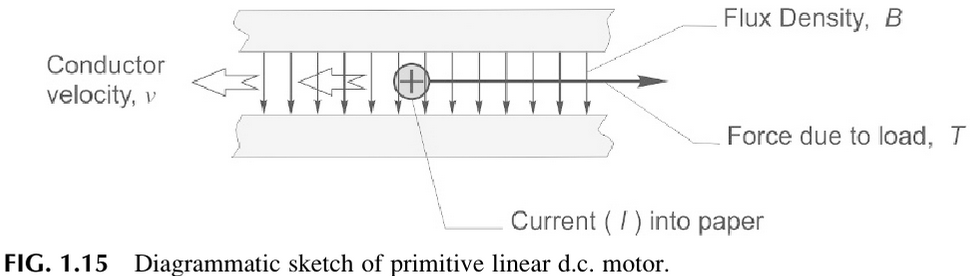
\includegraphics[width=0.53\linewidth]{../../figures/HD-fig1_15.png}
\end{center}

The electromagnetic force  in a conductor is \alert{proportional to the current} and \alert{the strength of the magnetic field}:
\[F=k_mI=(Bl_m)I,\] where \(B\) is the magnetic flux density in the gap, \(I\) is the current, an \(l_m\) is the length of the conductor. 

\alert{Activity} In a large motor of \unit{4}{\mega\watt} with an axial length of \(l_m=\unit{2}{\meter}\), the magnetic flux density is \(B=\unit{0.8}{\tesla}\) and the current is \(I=\unit{3}{\kilo\ampere}\). How many parallel conductors are needed to achieve a force of \(F=\unit{259.2}{\kilo\newton}\)?
\end{frame}

\begin{frame}[label={sec:org30e5cc4}]{The two equations of the DC motor}
\begin{block}{The force on the electrical conductor in the magnetic field}
\[ F(t) = k_m i(t) \quad\Leftrightarrow\quad T(t) = k_m r i(t),\]
where \(r\) is the radius of the motor.
\end{block}

\begin{block}{Voltage generated in a conductor that moves in a magnetic field}
\[ e(t) = k_v v(t) \quad\Leftrightarrow\quad e(t) = k_v r \omega(t)\]
\(e(t)\) is called  \emph{Back electro-motive force (Back e.m.f.)}.
\end{block}
\end{frame}

\begin{frame}[label={sec:org41407f8}]{Electrical and mechanical power}
\begin{center}
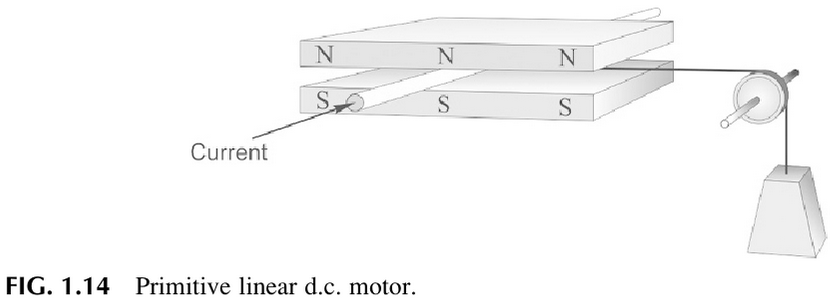
\includegraphics[width=0.4\linewidth]{../../figures/HD-fig1_14.png}
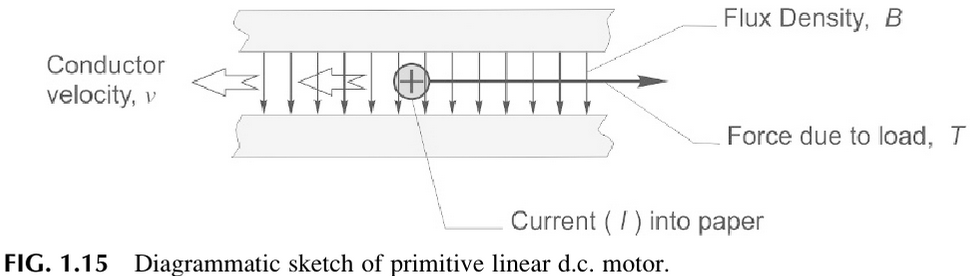
\includegraphics[width=0.53\linewidth]{../../figures/HD-fig1_15.png}
\end{center}

With constant velocity \(v\) and ignoring friction and electrical resistance: 

\[ \text{Electromagnetic force} = \text{Mechanical force} \quad\Leftrightarrow\quad F=k_mI =Bl_mI = mg\]
\[ \text{Electric power} = \text{Mechanical power} \quad \Leftrightarrow\quad \underbrace{V_1I}_{P_e} = \underbrace{Fv = Bl_mI v}_{P_m} \] 
It is necessary to apply a voltaje \(V_1\) across the cable to maintain the current \(I\). \alert{This voltage is equal to the back e.m.f.} 
\[ V_1I = Bl_mIv \quad \Rightarrow \quad V_1 = (Bl_m)v = k_v v = \tikz[baseline = 0.1ex]{\node[red, circle, draw, inner sep=3pt, pin={[red]0:{Back e.m.f.}}] at (0, 0.1 cm) {\textcolor{black}{E}}}\]

\alert{Actividad} What is the relationship between the two constants \(k_v\) and \(k_m\)?
\end{frame}

\begin{frame}[label={sec:org6bcdbea}]{Electrical and mechanical power}
In practice some energy is lost due to the resistance in the electrical circuit.
\begin{align*}
\text{Electrical power drawn} &= \text{Heat production} + \text{Mechanical power}\\
V_2 I &= RI^2 + EI
\end{align*}
Where \(V_2 > V_1 = (Bl_m)v = E\).

The efficiency of the motor

\[ \text{efficiency} = \frac{\text{Mechanical power}}{\text{Electrical power drawn}} = \frac{EI}{V_2I} = \frac{E}{RI + E}\]

\alert{Activity} An electri motor has a motor constant \(k=\unit{0.05}{\kilo\newton\per\ampere}\) and an armature resistance  of \(R=\SI{2}{\milli\ohm}\). It is producing a mechanical power of \unit{4}{\mega\watt} at a velocity of \(v=\unit{10}{\meter\per\second}\). Calculate the back e.m.f \(E\), the current \(I\), then voltage \(V_2\) and the efficiency.
\end{frame}

\begin{frame}[label={sec:orgfedfd90}]{Rotation}
\begin{center}
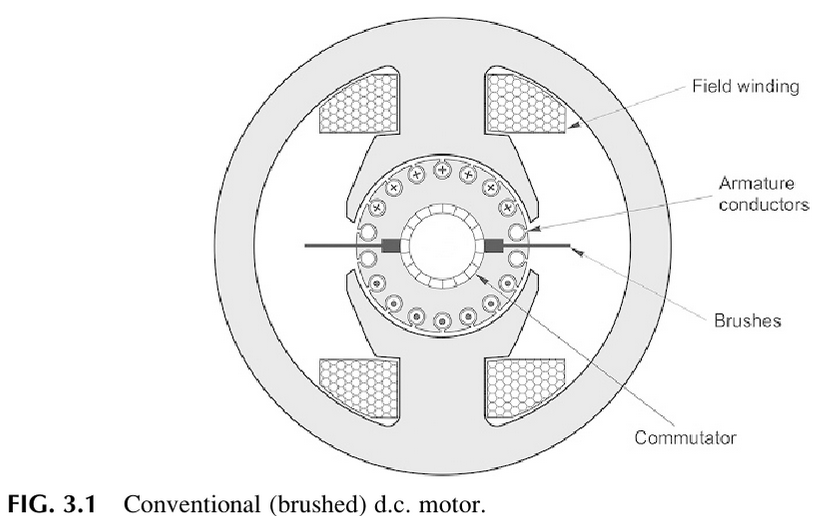
\includegraphics[width=0.4\linewidth]{../../figures/HD-fig3_1.png}
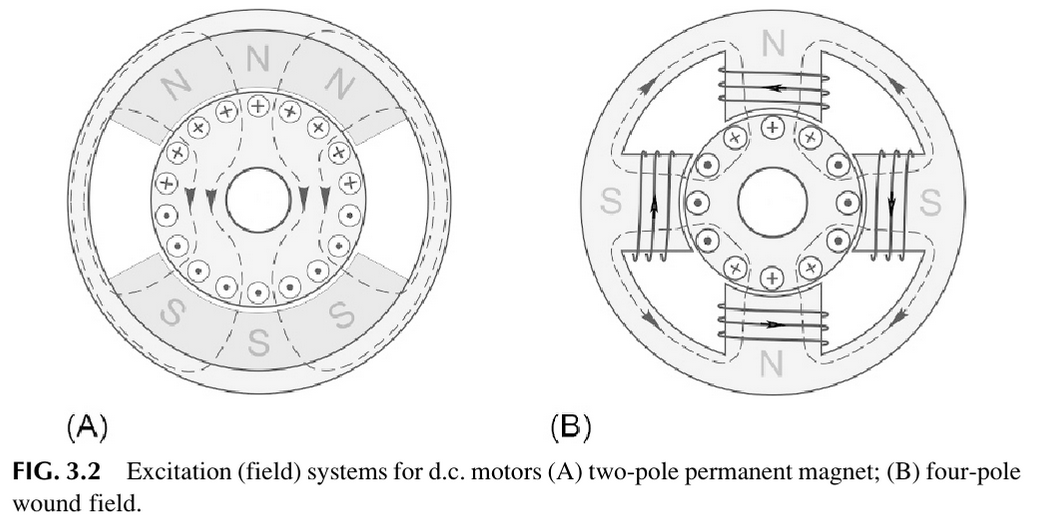
\includegraphics[width=0.53\linewidth]{../../figures/HD-fig3_2.png}
{\footnotesize Source: Hughes and Drury}
\end{center}
\end{frame}

\begin{frame}[label={sec:org75303af}]{Equivalent circuit}
\begin{center}
  \begin{circuitikz}
    \draw (4,1) node[elmech](motor){M};
    \draw (motor.north) to[R=$R$] (4,4) to[L=$L$] (0,4)
    to[american voltage source, label=$V$] (0,0) -| (motor.south);
    \draw[thick,->>](motor.right)--++(1,0)node[midway,above]{$\omega$};

    \node[] at (2, -0.8 cm) {\(L \frac{d}{dt}i(t) +  Ri(t) + k\omega(t) = V\)};

    \begin{scope}[xshift=8cm]
    \draw (4,1) node[elmech](motor){M};
    \draw (motor.north) to[R=$R$] (4,4) to[short] (0,4)
    to[american voltage source, label=$V$] (0,0) -| (motor.south);
    \draw[thick,->>](motor.right)--++(1,0)node[midway,above]{$\omega$};
    \node[] at (2, -0.8 cm) {\(Ri(t) + k\omega(t) = V\)};
    \end{scope}
  \end{circuitikz}
\end{center}

\begin{center}
Newton: \(J\frac{d}{dt}\omega(t) = ki(t) - T_l(t)\)
\end{center}
\end{frame}


\begin{frame}[label={sec:org0c4bdbf}]{Velocity with constant load}
\begin{align}
L\frac{d}{dt}i(t) + Ri(t) + k\omega(t) &= V(t)\\
J\frac{d}{dt}\omega(t) &= ki(t) - T_l(t)
\end{align}

In steady-state: \(i(t) = I\), \(\omega(t) = \omega\).

\begin{align}
RI + k\omega &= V\\
0 &= kI - T_l
\end{align}

\alert{Activity} Write the angular velocity as function of the load \(T_l\) and the volage \(V\)
\[\omega = f(V, T_l) = \frac{V}{k} - \frac{RT_l}{k^2}\]
\end{frame}

\begin{frame}[label={sec:org867c932}]{Velocity with constant load}
\[\omega = f(V, T_l) = \frac{V}{k} - \frac{RT_l}{k^2}\]
A specific motor has a motor constant \(k=\unit{4}{\newton\meter\per\ampere}\) and armature resistence \(R=\SI{1}{\ohm}\). A voltage of \(V=\unit{100}{\volt}\) is applied over the armature circuit.


\alert{Activity} Sketch how the steady-state velocity depends on the load \(T_l\). What is the stall torque (the torque that will cause the motor to stand still)?

\begin{center}
  \begin{tikzpicture}[xscale=0.8]
    \draw[->] (0, 0) -- (9, 0) node[right] {$T_l$ [\unit{}{\newton\meter}]};
    \draw[->] (0, 0) -- (0, 3) node[left] {$\omega$};
    \foreach \t in { 1, 2, ..., 8} {
    \draw (\t, 0) -- (\t, -0.1) node[below] {\t{}00};
    }
    \end{tikzpicture}

\end{center}
\end{frame}

\begin{frame}[label={sec:org6d77004}]{Start-up}
For a motor that is not rotating, the back e.m.f is zero, and only the resistance and the inductance of the armature limits the current.

\begin{center}
  \begin{circuitikz}
    \draw (4,1) node[elmech](motor){M};
    \draw (motor.north) to[R=$R$] (4,4) to[L=$L$] (0,4)
    to[american voltage source, label=$V$] (0,0) -| (motor.south);
    \draw[thick,->>](motor.right)--++(1,0)node[midway,above]{$\omega$};

    \node[] at (2, -0.8 cm) {\(L \frac{d}{dt}i(t) +  Ri(t) + k\omega(t) = V\)};
  \end{circuitikz}
\end{center}


It is necessary to be careful with applying too much voltage at start-up to avoid excessive current in the motor.
\end{frame}

\section{Modeling}
\label{sec:org194e549}
\begin{frame}[label={sec:org4bc2bbd}]{Block-diagram of the equivalent circuit}
\begin{center}
  \begin{circuitikz}
    \draw (4,1) node[elmech](motor){M};
    \draw (motor.north) to[R=$R$] (4,4) to[L=$L$] (0,4)
    to[american voltage source, label=$V$] (0,0) -| (motor.south);
    \draw[thick,->>](motor.right)--++(1,0)node[midway,above]{$\omega$};

    \node[] at (9, 2 cm) {\(L \frac{d}{dt}i(t) +  Ri(t) + k\omega(t) = V\)};
    \node[] at (9, 1 cm) {\(\frac{d}{dt}i(t) = \frac{1}{L} \Big(-Ri(t) - k\omega(t) + V\Big)\)};
  \begin{scope}[yshift=-15mm, xshift=8cm,
  block/.style={rectangle, draw, minimum width=12mm, minimum height=10mm},
  amp/.style = {regular polygon, regular polygon sides=3,
        draw, fill=white, text width=1em,
        inner sep=1pt, outer sep=0mm,
        shape border rotate=-90},
	summ/.style = {circle, draw, inner sep = 1pt},]
   \node[block,] (int) at (0,0) {$\int$};
   \node[amp, left of=int, node distance=30mm] (oneoverL) {$\frac{1}{L}$}; 
   \draw[->] (oneoverL) -- node[above] {$\frac{d}{dt}i(t)$} (int);
   \node[summ, left of=oneoverL, node distance=20mm] (sum) {\small $\Sigma$};
   \node[coordinate, left of=sum, node distance=30mm] (Vin) {};
   \draw[->] (Vin) -- node[above, near start] {$V$} node[coordinate, pos=0.6] (mp) {} (sum);
   \node[amp, above of=mp, node distance=15mm] (mkonst) {$-k$};
   \end{scope}
  \end{circuitikz}
  \end{center}
\end{frame}
\end{document}